\documentclass[default]{beamer}
\setbeamertemplate{navigation symbols}{}

\usetheme{CambridgeUS}
\useoutertheme{infolines}
%\usecolortheme{crane}

\usepackage{cmap}							% Поддержка поиска русских слов в PDF (pdflatex)
\usepackage[T2A]{fontenc}       			%поддержка кириллицы
\usepackage[utf8]{inputenc}					% Выбор языка и кодировки
\usepackage[english, russian]{babel}
\usepackage{tikz}
\usetikzlibrary{calc}

\graphicspath{{../../images/}} 			% Пути к изображениям

\makeatletter
\setbeamertemplate{footline}
{
	\leavevmode%
	\hbox{%
		\begin{beamercolorbox}[wd=.333333\paperwidth,ht=2.25ex,dp=1ex,center]{author
				in head/foot}%
			\usebeamerfont{author in
				head/foot}\insertshortauthor~~\beamer@ifempty{\insertshortinstitute}{}{(\insertshortinstitute)}
		\end{beamercolorbox}%
		\begin{beamercolorbox}[wd=.333333\paperwidth,ht=2.25ex,dp=1ex,center]{title in
				head/foot}%
			\usebeamerfont{title in head/foot}\insertshorttitle
		\end{beamercolorbox}%
		\begin{beamercolorbox}[wd=.333333\paperwidth,ht=2.25ex,dp=1ex,right]{date in
				head/foot}%
			\usebeamerfont{date in head/foot}\insertshortdate{}\hspace*{2em}
			\insertframenumber{}\hspace*{2ex} 
		\end{beamercolorbox}
	}%
	\vskip0pt%
}

\let\Theorem\relax
\newtheorem{Theorem}{Теорема}
\newtheorem{Def}{Определение}

\begin{document}
	
	\title[Perception and HTM]{Иерархическая временная память как модель восприятия и её автоматное представление}
	\author[Панов]{Александр Панов}
	\institute[ИСА РАН]{ИСА РАН}
	\date{17 июня 2015~г.} 
	
	\begin{frame}
		\titlepage
	\end{frame}
	
	\begin{frame}
		\frametitle{Модели когнитивных функций}
		
		Использование моделей простейших когнитивных функций, таких как восприятие и сопоставление с образцом:
		\begin{itemize}
			\item в целях построения более совершенных алгоритмов распознавания объектов, сложных сцен и движений (глубокие нейронные сети),
			\item в целях формирования базиса для построения моделей более сложных когнитивных функций, таких как целеполагание и планирование поведения.
		\end{itemize}
	\end{frame}

	\begin{frame}
		\frametitle{Цели работы}
		
		Высшие когнитивные функции оказывается возможным описывать с использованием знаковой картины мира. Формализация понятия знака позволяет строить алгоритмы целеполагания, планирования поведения и распределения ролей в коллективе.
		\par\bigskip
		Цель "--- построить модель процесса образования и функционирования основных компонент знака, которая соответствовала бы современным представлениям нейрофизиологов о функционировании этих компонент.
		\begin{center}
			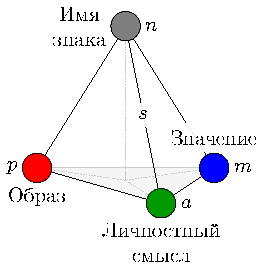
\includegraphics[width=0.27\textwidth]{signs/sign_colored}
		\end{center}
		
	\end{frame}

	\begin{frame}
		\frametitle{Модели восприятия}
		
		Биологически (нейрофизиологически) правдоподобная модель восприятия позволит формально описать процесс работы компонент образа и значения знака.
		\par\bigskip
		Имеющиеся работы:
		\begin{itemize}
			\item временная хеббовсккая самоорганизующаяся карта (THSOM, Кутник),
			\item адаптивная запоминающе-предсказывающая структура (AMPF, Ролинсон и Ковадло),
			\item система адаптивного резонанса (ART, Гроссберг),
			\item иерархическая временная память (HTM, Хокинс и Георг).
		\end{itemize}
	\end{frame}

	\begin{frame}
		\frametitle{Нейронный субстрат}
		
		\begin{columns}
			\begin{column}{0.5\textwidth}
				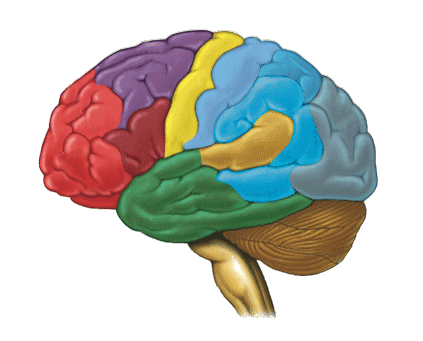
\includegraphics[width=0.7\textwidth]{phisio/mozg_2}
				\par\bigskip
				\hspace{-7mm}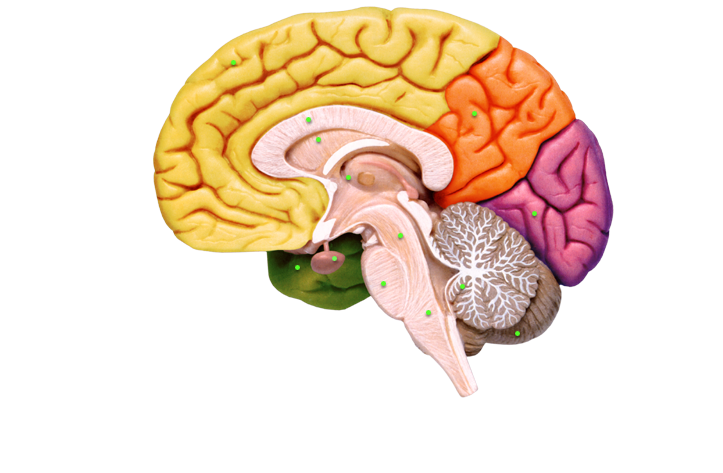
\includegraphics[width=0.9\textwidth]{phisio/mozg}
			\end{column}
			\begin{column}{0.5\textwidth}
				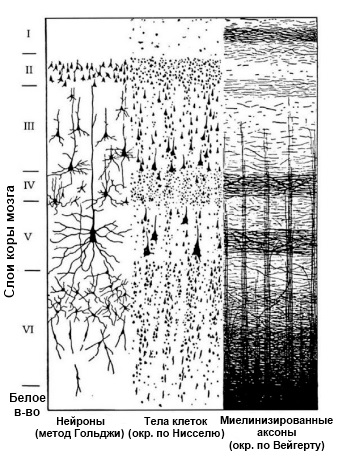
\includegraphics[width=0.9\textwidth]{phisio/column_layers_ru}
			\end{column}
		\end{columns}
	\end{frame}

	\begin{frame}
		\frametitle{Основные свойства модели и используемые упрощения}
		
		\begin{columns}
			\begin{column}{0.3\textwidth}
				\begin{figure}
					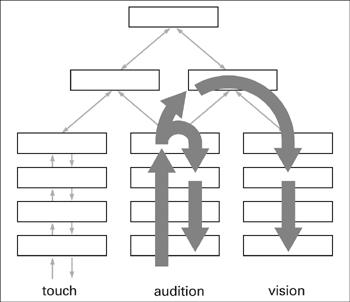
\includegraphics[width=\textwidth]{info_flow.jpg}
				\end{figure}
			\end{column}
			\begin{column}{0.7\textwidth}
				\begin{overlayarea}{\textwidth}{0.7\textheight}
					\only<1>{
						Принимается следующие гипотезы:
						\begin{itemize}
							\item неокортекс состоит из зон (регионов), состоящих в свою очередь из колонок и имеющих одинаковое строение на всех участках коры;
							\item колонки в регионе объединены латеральными связями;
							\item таламус формирует последовательности паттернов за счет задержки возбуждения/торможения.
						\end{itemize}
					}
					
					\only<2>{
						Основные свойства:
						\begin{itemize}
							\item хранение последовательности паттернов в инвариантной форме,
							\item воспроизведение паттернов автоассоциативно,
							\item хранение паттернов в иерархической системе,
							\item использование обратной связи для предсказания поступающей на данный уровень иерархии информации. 
						\end{itemize}
					}
					
					\only<3>{
						Упрощения:
						\begin{itemize}
							\item дискретность во времени,
							\item простейшая строгая иерархия со связями только между
							ближайшими уровнями,
							\item гипотеза одинаковой длительности распознаваемых явлений в рамках одного региона,
							\item пороговая модель принятия решений в случае неопределенности результата распознавания,
							\item подавление непредвиденного сигнала,
							\item отсутствие моторной составляющей обратной связи.
						\end{itemize}
					}				
				\end{overlayarea}
			\end{column}
		\end{columns}
	\end{frame}

	\begin{frame}
		\frametitle{Формальная модель нейрона}
		
		\begin{center}
			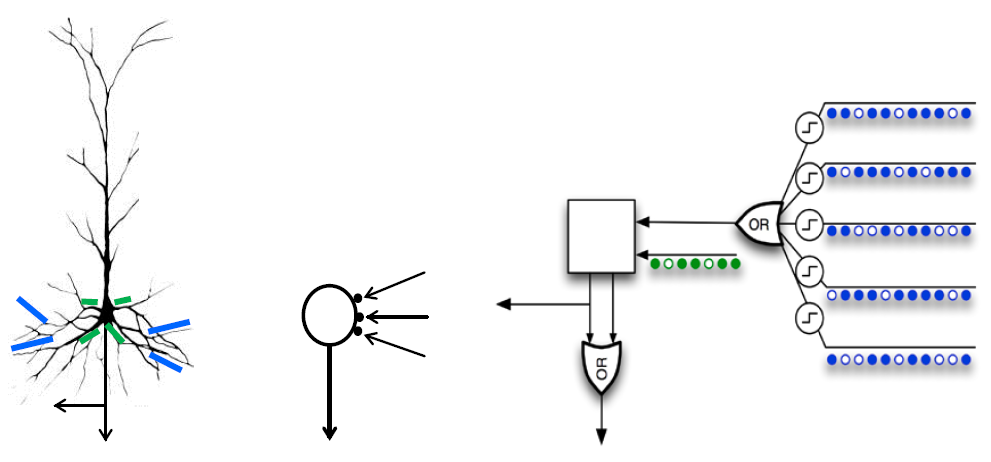
\includegraphics[width=0.9\textwidth]{phisio/neuro_htm}
		\end{center}
		
		\begin{itemize}
			\item Проксимальный дендритный сегмент "--- прямая активация.
			\item Дистальные дендритные сегменты "--- латеральный вход и состояние предсказания.
		\end{itemize}
	\end{frame}

	\begin{frame}
		\frametitle{Иерархическая организация нейронов}
		
		\begin{columns}
			\begin{column}{0.5\textwidth}
				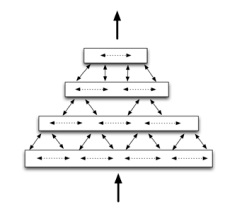
\includegraphics[width=0.9\textwidth]{mpf/hierarchy}
			\end{column}
			\begin{column}{0.5\textwidth}
				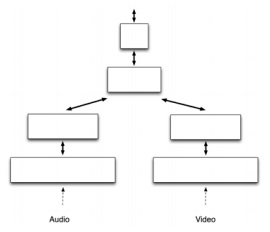
\includegraphics[width=0.9\textwidth]{mpf/hierarchy_conv}
			\end{column}
		\end{columns}

	\end{frame}

	\begin{frame}
		\frametitle{Иерархическая модель}
		

		\begin{overlayarea}{\textwidth}{\textheight}
			\only<1>{
				\begin{center}
					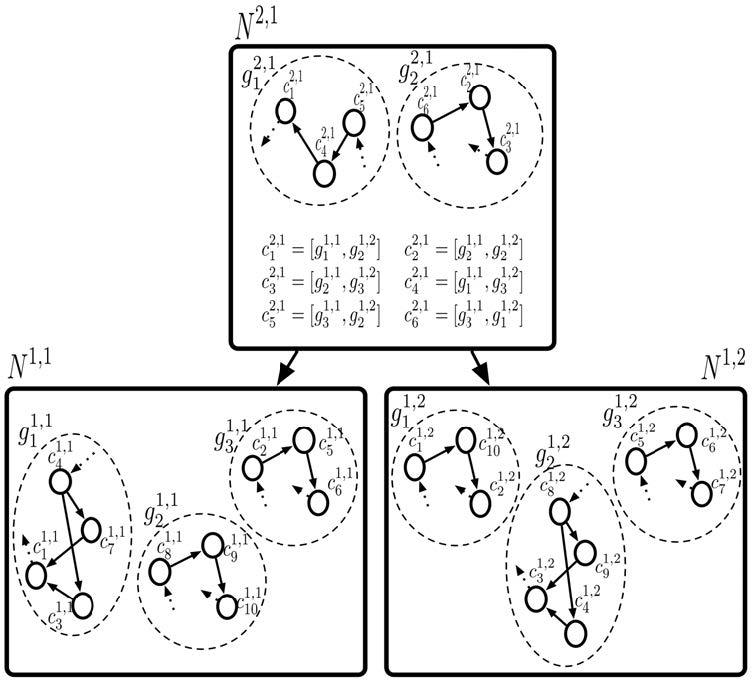
\includegraphics[width=0.7\textwidth]{hawkins_htm}
				\end{center}
			}
			\only<2>{
				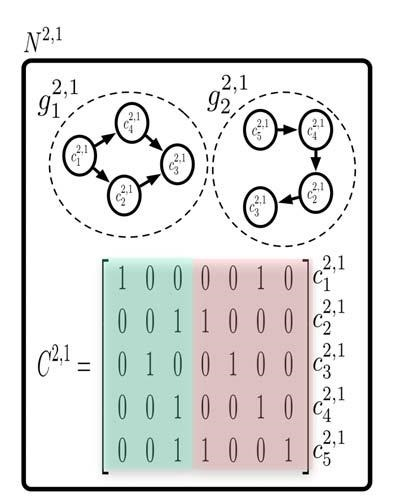
\includegraphics[width=0.4\textwidth]{hawkins_htm_ex_a}
				\hspace{20mm}
				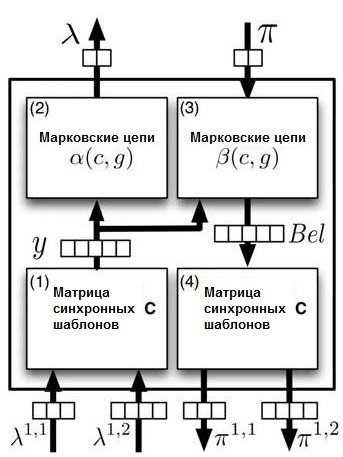
\includegraphics[width=0.4\textwidth]{hawkins_htm_ex_b}
			}
		\end{overlayarea}
	\end{frame}

	\begin{frame}
		\frametitle{Послойная организация}
		
		\begin{columns}
			\begin{column}{0.65\textwidth}
				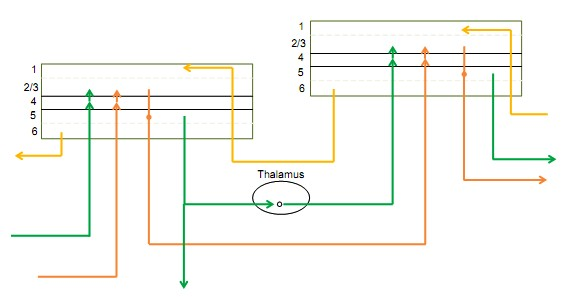
\includegraphics[width=0.9\textwidth]{regions_connect}
			\end{column}
			\begin{column}{0.35\textwidth}
				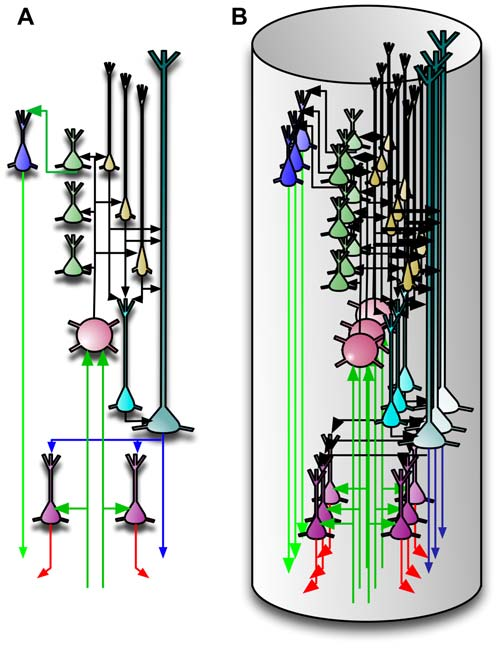
\includegraphics[width=\textwidth]{column}
			\end{column}
		\end{columns}
	\end{frame}

	\begin{frame}
		\frametitle{Образная компонента знака}
		
		При окончании процесса обучения синапсы определяют как вертикальные связи между узлами, так и горизонтальные связи в рамках одного узла.
		\par\bigskip
		Далее будет рассмотрена автоматная модель процесса восприятия, на основе которой будут определены образная компонента знака. 
		\par\bigskip
		Каждому узлу будет соответствовать специальный распознающий автомат, состояния которого были сформированы в результате процесса обучения по алгоритму HTM.
	\end{frame}
	
	\begin{frame}
		\frametitle{Признаки и распознающие автоматы}
		Для уточнения постановки задачи введём следующие объекты:
		\begin{itemize}
			\item 
			$\mathcal R$ "--- совокупность распознающих автоматов или $R$-автоматов вида $<A,Q,B,\varphi,\eta>$ с множествами входов $A$, выходов $B$ и состояний $Q$ и определёнными в соответствии с нейрофизиологическими данными функциями переходов $\varphi$ и выходов $\eta$,
			\item
			$\mathcal F$ "--- совокупность допустимых признаков.
		\end{itemize}
		\par\bigskip
		Введём бинарное отношение $\dashv$ и будем читать $f_k{\dashv}R_i^j$ как <<признак $f_k$ распознаётся $R$-автоматом $R_i^j$>>. 
	\end{frame}
	
	\begin{frame}
		\frametitle{Иерархия распознающих автоматов}
		\begin{figure}
			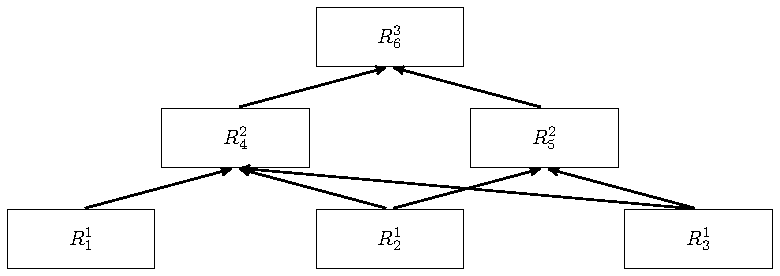
\includegraphics[width=0.5\textwidth]{rb_hierarchy}
		\end{figure}
		Представим иерархию $R$-автоматов в виде связного ориентированного ярусного графа $G_R=(V,E)$:
		\begin{itemize}
			\item 
			$V=\mathcal R$ "--- множество вершин,
			\item
			$E\subset \mathcal R\times\mathcal R$ "--- множество рёбер,
			\item 
			каждая вершина, принадлежащая $j$-ому ярусу графа $G_R$, является $R$-автоматом $R_i^j$ уровня $j$,
			\item
			каждое ребро $e=(R_i^j,R_k^{j+1}){\in}E$ обозначает иерархическую связь между дочерним $R$-автоматом $R_i^j$ и $R$-автоматом "--- родителем $R_k^{j+1}$.				
		\end{itemize}
	\end{frame}
	
	\begin{frame}
		\frametitle{Входные признаки и функции распознавания}
		Введём следующие определения.
		\begin{itemize}
			\item 
			Признак $f\dashv R_k^{j-1}$ называется входным для $R$-автомата $R_i^j$, если $R_k^{j-1}$ является дочерним автоматом по отношению к $R_i^j$. Всё множество входных признаков для $R_i^j$ будем обозначать $F_i^j$.
			\item
			Для каждого признака $f^*{\in}F_i^{*j}$ введём \textit{функцию распознавания} $\hat{f}(x_1,\dots,x_q)=x^*$, где $x^*{\in}(0,1)$ "--- вес распознаваемого признака $f^*$, а $x_1,\dots,x_q{\in}(0,1)$ "--- веса признаков из множества входных признаков $F_i^j$. Всю совокупность функций распознавания для $R_i^j$ будем обозначать $\hat{F}_i^j$.
			\item Каждой функции распознавания $\hat{f}_k$ из множества $\hat F_i^j$ поставим в соответствие набор булевых матриц предсказания $Z_k=\{Z_1^k,…,Z_m^k\}$ размерности $q\times h$, множество которых $\mathcal Z_i^j$ формирует состояния $R$-автомата.
		\end{itemize}
	\end{frame}
	
	\begin{frame}
		\frametitle{Алгоритм $\mathfrak A_{th}$ вычисления автоматной функции}
		
		\begin{tikzpicture}[overlay,remember picture]
		
		\tikzstyle{z_matrix} = [draw, rectangle, minimum width = 60, minimum height = 60,fill=white];
		
		\onslide<1->{
			\node (meas_fun) at (0.7,0.5) {$\hat f_1,\hat f_2\dots,\hat f_k$};	
		}
		\onslide<2->{
			\node (control_vect) at ($(meas_fun)+(-0.5,1.2)$) {$\hat x^{j+1}$};
			\path[->,thick,red] (control_vect.east)  edge[out = -45, in = 45, right] (meas_fun.north); 
		}
		\onslide<3->{
			\node[z_matrix] (z_1) at ($(meas_fun)+(2.6,-0.5)$) {};
			\node[z_matrix] at ($(z_1)+(0.2,-0.1)$) {};
			\node[z_matrix] at ($(z_1)+(0.4,-0.2)$) {};
			
			\node[z_matrix] at ($(z_1)+(0.9,-0.5)$) {};
			\node[z_matrix] at ($(z_1)+(1.1,-0.6)$) {};
			\node[z_matrix] at ($(z_1)+(1.3,-0.7)$) {};
			
			\path[->,thick,blue] ([xshift=20]meas_fun.south)  edge[out = -90, in = -155, right] ($(z_1)+(-1,-1.2)$);
			\path[->,thick,blue] ([xshift=-25]meas_fun.south)  edge[out = -90, in = -155, right] ($(z_1)+(-0.1,-1.7)$);
			
			\node at ($(z_1)+(-1,1.4)$) {$Z^*$};
			
			\node at ($(z_1)+(0.8,1.4)$) {$Z_1$};
			\node at ($(z_1)+(1.4,1.2)$) {$\ddots$};
			\node at ($(z_1)+(2,0.9)$) {$Z_k$};
		}
		
		\onslide<4->{
			\draw[ultra thick, green!60!black] ($(z_1)+(-0.4,-1.1)$) -- ($(z_1)+(-0.4,0.6)$);
			\draw[ultra thick, green!60!black] ($(z_1)+(0.5,-1.6)$) -- node[right,black] {$z_1^r$} ($(z_1)+(0.5,0.1)$);
			
			\draw[->, thick, green!60!black] ($(z_1)+(-0.1,-3)$) -- node[right,black] {$\bar x(0)$} ($(z_1)+(-0.1,-2)$);
		}
		
		\onslide<5->{
			\node[z_matrix] (z_2) at ($(z_1)+(5,0)$) {};
			\node[z_matrix] at ($(z_2)+(0.2,-0.1)$) {};
			
			\node[z_matrix] at ($(z_2)+(0.9,-0.5)$) {};
			\node[z_matrix] at ($(z_2)+(1.3,-0.7)$) {};
			
			\node at ($(z_2)+(-1,1.4)$) {$Z^*$};
			\node at ($(z_2)+(0.8,1.4)$) {$Z_1$};
			\node at ($(z_2)+(1.4,1.2)$) {$\ddots$};
			\node at ($(z_2)+(2,0.9)$) {$Z_k$};
			
			\draw[->, ultra thick] ($(z_1)+(2.6,-0.6)$) -- node [above] {\scriptsize$\frac{\|\bar z_1^r-\bar x(0)\|}{\|\bar z_1^r\|+\|\bar x(0)\|}$} ($(z_1)+(3.7,-0.6)$);
			
			\draw[ultra thick, dotted, green!60!black] ($(z_2)+(-0.6,-1)$) -- ($(z_2)+(-0.6,0.7)$);
			\draw[ultra thick, dotted, green!60!black] ($(z_2)+(0.5,-1.6)$) -- ($(z_2)+(0.5,0.1)$);
		}
		
		
		\onslide<6->{
			\draw[->, thick, red] ($(z_2)+(0.3,1.4)$) -- node[right,black] {$\bar x^*(0)$} ($(z_2)+(0.3,3)$);
		}
		
		\onslide<7>{
			\draw[<-, thick, red] ($(z_2)+(-0.1,-3)$) -- node[right,black] {$\hat x^j(0)$} ($(z_2)+(-0.1,-2)$);
		}
		
		\onslide<7->{				
			\draw[ultra thick, green!60!black] ($(z_2)+(-0.4,-1)$) -- ($(z_2)+(-0.4,0.7)$);
			\draw[ultra thick, green!60!black] ($(z_2)+(0.7,-1.6)$) -- node[right,black] {$z_2^r$} ($(z_2)+(0.7,0.1)$);	
		}
		\onslide<8->{
			\draw[->, thick, green!60!black] ($(z_2)+(-0.1,-3)$) -- node[right,black] {$\bar x(1)$} ($(z_2)+(-0.1,-2)$);
		}
		
		\onslide<9->{
			\draw[->, ultra thick] ($(z_2)+(2.6,-0.6)$) -- node [above] {\scriptsize$\frac{\|\bar z_1^r-\bar x(1)\|}{\|\bar z_1^r\|+\|\bar x(1)\|}$} ($(z_2)+(3.7,-0.6)$);
		}
		\end{tikzpicture}
	\end{frame}
	
	\begin{frame}
		\frametitle{Корректность алгоритма $\mathfrak A_{th}$}
		
		Оказывается, что алгоритм $\mathfrak A_{th}$ является корректным с точки зрения теории распознавания, т.~е. с помощью него могут быть правильно классифицированы любые корректные поступающие сигналы. При этом он корректен как в статическом случае, так и в динамическом. 
		\par\bigskip
		Оказывается, что корректной является работа и всей иерархии распознающих автоматов.
	\end{frame}

	\begin{frame}
		\frametitle{Эксперименты по распознаванию последовательностей}

		\begin{center}
			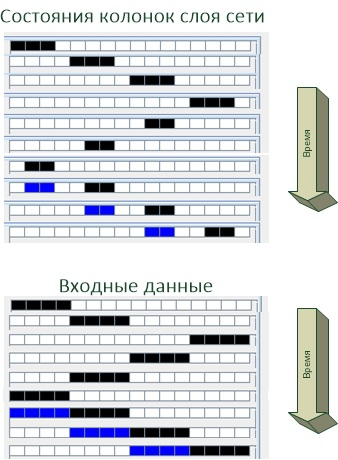
\includegraphics[width=0.4\textwidth]{mpf/experiments}
		\end{center}
		
	\end{frame}
		
	\begin{frame}
		\frametitle{Формирование пары <<образ "--- значение>>}
		
		Применим введённые понятия для решения задачи формирования пары <<образ "--- значение>> элемента картины мира субъекта.
		\par\bigskip
		Уточним постановку задачи.
		
		\begin{figure}
			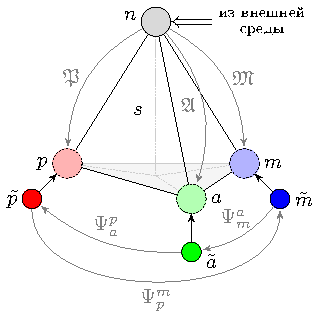
\includegraphics[width=0.45\textwidth]{signs/sign_naming_colored}
		\end{figure}
	\end{frame}
	
	\begin{frame}
		\frametitle{Отношение поглощения признаков}
		Введём семейство бинарных отношений $\{\sqsubset,\sqsubset^1,\sqsubset^2,\dots\}$, определённых на декартовом произведении $\mathcal F\times\mathcal F$. 
		\par\bigskip
		\begin{columns}
			\begin{column}{0.6\textwidth}
				Признак $f_1$ поглощается признаком $f_2$: $f_1\sqsubset f_2$, в том случае, если $f_1\dashv R_i^j, f_2\dashv R_k^{j+1}$, $R_k^{j+1}$ "--- родительский $R$-автомат по отношению к $R_i^j$ и в множестве матриц предсказания $Z_2$ признака $f_2$ существует как минимум одна матрица $Z_r^2$, содержащая некоторый столбец $\bar z_u^r$ с элементом $z_{uv}^r\not=0$, где $v$ "--- индекс признака $f_1$ во входном векторе для $R$-автомата $R_2^{j+1}$.
			\end{column}
			\begin{column}{0.4\textwidth}
				\begin{figure}[t]
					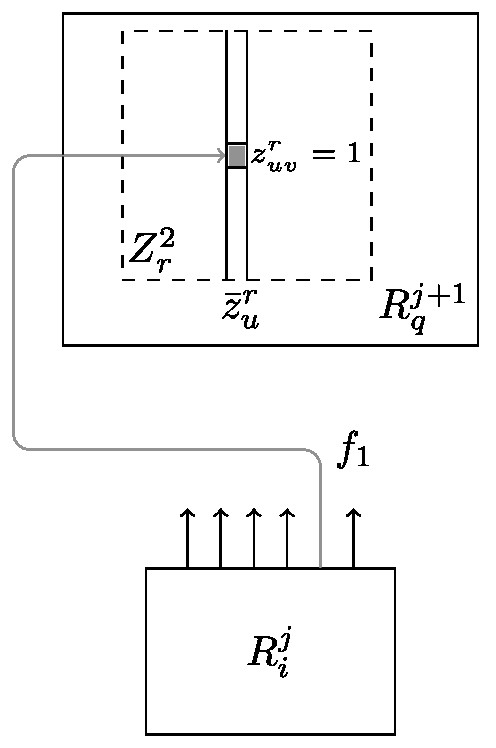
\includegraphics[width=0.75\linewidth]{automata/meas}
				\end{figure}
			\end{column}
		\end{columns}
	\end{frame}
	
	\begin{frame}
		\frametitle{Процедурные и объектные признаки}
		Значение знака будем рассматривать как множество правил, каждое из которых соответствует некоторому действию. Правило для простоты будем представлять в виде пары <<условия "--- эффект действия>> так,~как это принято в искусственном интеллекте. 
		\par\bigskip
		Введём операцию $\Lambda$, которая по множеству матриц распознавания $\mathcal Z_k$ признака $f_k$ определяет два набора индексов столбцов матриц из $Z_k$. Первый набор $I_c=\{i_1^c,i_2^c,\dots\}$, $\forall k\ 0\leqslant i_k^c < h$, составляют индексы \textit{столбцов условий}, в которых ненулевые элементы определяют условия проявления признака $f_k$. Второй набор $I_e=\{i_1^e,i_2^e,\dots\}$, $\forall k\ 0\leqslant i_k^e < h$, состоит из индексов  \textit{столбцов эффектов}, в которых ненулевые элементы определяют эффекты проявления признака $f_k$. 
		
	\end{frame}
	
	\begin{frame}
		\frametitle{Процедрные и объектные признаки}
		
		\begin{Def}
			Признаки, для матриц предсказания которых процедура $\Lambda$ выдаёт непустые множества индексов $I_c$ и $I_e$, будем называть процедурными признаками, остальные "--- объектными признаками.
		\end{Def}
		\par\bigskip
		Пополним семейство отношений $\{\sqsubset,\sqsubset^1,\sqsubset^2,\dots\}$ двумя отношениями: $\sqsubset^c$ и $\sqsubset^e$, принадлежность к которым пары признаков $(f_1,f_2)$ свидетельствует о том, что признак $f_1$ присутствует соответственно в столбце условий и эффектов как минимум в одной матрице предсказания процедурного признака $f_2$.
	\end{frame}
	
	\begin{frame}
		\frametitle{Образ знака}
		
		Пусть $S$ "--- множество знаков. Будем считать, что между множествами $S$ и $\mathcal F$ установлено некоторое взаимно-однозначное соответствие.
		
		\begin{Def}
			Если $f_1$ "--- признак, соответствующий знаку $s_1$, то подмножество $\tilde p(f_1)\subset\mathcal F$ таких признаков, что $\forall f_i\in\tilde p(f_1) f_i\sqsubset f_1$, будем называть образом знака $s_1$ (признака $f_1$).
		\end{Def}
		
		На множестве всех образов $\tilde P$ можно ввести метрику $\rho_p(\tilde p(f_1),\tilde p(f_2))$.
	\end{frame}
	
	\begin{frame}
		\frametitle{Значение знака}
		\begin{Def}
			Если $f_1$ "--- признак, соответствующий знаку $s_1$, $f_2$ "--- процедурный признак и $f_1\sqsubset^c f_2$, то будем называть $f_2$ элементом значения знака $s_1$ (признака $f_1$). Множество всех элементов значения признака $f_1$ будем обозначать $\tilde m(f_1)$.
		\end{Def}
		
		На множестве всех значений $\tilde M$ можно ввести метрику $\rho_m(\tilde m(f_1),\tilde m(f_2))$.
	\end{frame}
	
	\begin{frame}
		\frametitle{Процедурный признак как правило}
		Любой элементарный процедурный признак $f_p$, распознаваемый $R$-автоматом $R$, можно представить в виде правила $r_p=<F_C(f_p),F_A(f_p),F_D(f_p)>$, в котором:
		\begin{itemize}
			\item $F_C (f_p )\subseteq F_i^j$ "--- множество признаков "--- условий правила: $\forall f\in F_C(f_p)$ $f\sqsubset^c f_p$;
			\item $F_A(f_p)\subseteq F_i^j$ "--- множество добавляемых правилом признаков: $\forall f\in F_A(f_p)$ $f\sqsubset^e f_p,f\notin F_C$;
			\item $F_D(f_p)\subseteq F_i^j$ "--- множество удаляемых правилом признаков: $\forall f\in F_D(f_p)$ $f\notin F_A,f\in F_C$.
		\end{itemize}
	\end{frame}
	
	\begin{frame}
		\frametitle{Опыт наблюдения}
		Пусть опыт наблюдения субъекта записывается в виде функции $\Psi_p^m$. $\Psi_p^m(\tilde p)=\tilde m$, в том случае, если $\tilde p\in\tilde P$ является образом некоторого знака $s$, а $\tilde m\in\tilde M$ -- значением того же знака $s$.
		\par\bigskip
		Алгоритм $\mathfrak A_{pm}$ доопределения функции $\Psi_p^m$ обеспечивает формирование такого образа из множества признаков $\hat F$, при котором формируемое значение знака сходится к заданному значению $\tilde m^0=\{f_p^0\}$.
	\end{frame}
	
	\begin{frame}
		\frametitle{Алгоритм $\mathfrak A_{pm}$ формирования образа и значения}
		
		\begin{tikzpicture}[overlay,remember picture]
		
		\tikzstyle{z_matrix} = [draw, rectangle, minimum width = 60, minimum height = 60,fill=white];
		
		\onslide<1->{
			\node (start_f) at (0.3,0.5) {$\hat F$};	
			\node (etal_m) at (0.7,1.5) {$\tilde m^0=\{f_p^0\}$};			
			\node (start_m) at (0.3,2.5) {$\tilde M$};
			\node (build_p) at (0.7,-0.5) {$\tilde p^{(0)},\tilde m^{(0)}$};
		}
		\onslide<2->{
			\node (select_f) at ($(start_f)+(3,0)$) {$f$};
			\path[->,thick,red] (start_f.east)  edge[out = 10, in = 170, right] (select_f.west); 
			
			\node (p_t) at ($(select_f)+(0,-2.5)$) {$\tilde p^{(t+1)}$};
			\path[->,thick,red] (build_p.south)  edge[out = -45, in = 180, right] (p_t.west);
			\path[->,thick,red] (select_f.south)  edge[out = -90, in = 90, right] (p_t.north);
			
			\node[z_matrix] (z_f) at ($(start_f)+(4.5,-0.2)$) {};
			\node at ($(z_f)+(0,1.5)$) {$Z$};
			\draw[ultra thick, green!60!black] ($(z_f)+(-0.7,-0.8)$) -- ($(z_f)+(-0.7,0.8)$);
			\draw[ultra thick, green!60!black] ($(z_f)+(-0.4,-0.8)$) -- ($(z_f)+(-0.4,0.8)$);
			
			\draw[ultra thick, green!60!black] ($(z_f)+(0.7,-0.8)$) -- ($(z_f)+(0.7,0.8)$);
			\node[green!60!black] at ($(z_f)+(0.2,0)$) {$\cdots$};
			
		}
		\onslide<3->{
			\node (select_m) at ($(start_m)+(7,0)$) {$\tilde m(f_p^0)=\{f_p\}$};
			\path[->,thick,blue] (start_m.east)  edge[out = 10, in = 170, right] (select_m.west);
			
			\node[z_matrix] (z_m) at ($(z_f)+(4.5,0.5)$) {};
			\node at ($(z_m)+(0,1.5)$) {$Z_p$};
			\draw[ultra thick, green!60!black] ($(z_m)+(-0.6,-0.8)$) -- node[right,black] {$\bar z_1^c$} ($(z_m)+(-0.6,0.8)$);	
			\draw[ultra thick, green!60!black] ($(z_m)+(0.4,-0.8)$) -- node[right,black] {$\bar z_1^e$} ($(z_m)+(0.4,0.8)$);
		}
		\onslide<4->{
			\node[z_matrix] (z_mt) at ($(z_f)+(2,-3)$) {};
			\node at ($(z_mt)+(-0.5,1.5)$) {$Z_p^{(t+1)}$};
			
			\draw[ultra thick, green!60!black] ($(z_mt)+(-0.6,-0.8)$) -- ($(z_mt)+(-0.6,0.8)$);	
			\draw[ultra thick, green!60!black] ($(z_mt)+(0.4,-0.8)$) -- ($(z_mt)+(0.4,0.8)$);
			
			\path[->,thick,blue] (z_m.south) edge[out = -90, in = 90, right] (z_mt.north);
			\path[->,thick,blue] (build_p.east) edge[out = -20, in = 180, right] ([yshift=10]z_mt.west);
		}
		\onslide<5->{
			\node[z_matrix] (z_pt) at ($(z_m)+(1.5,-4)$) {};
			\node at ($(z_pt)+(0.7,1.5)$) {$Z^{(t+1)}$};
			
			\draw[ultra thick, green!60!black] ($(z_pt)+(-0.7,-0.8)$) -- ($(z_pt)+(-0.7,0.8)$);
			\draw[ultra thick, green!60!black] ($(z_pt)+(-0.4,-0.8)$) -- ($(z_pt)+(-0.4,0.8)$);
			
			\draw[ultra thick, green!60!black] ($(z_pt)+(0.7,-0.8)$) -- ($(z_pt)+(0.7,0.8)$);
			\node[green!60!black] at ($(z_pt)+(0.2,0)$) {$\cdots$};
			
			\path[->,thick,blue] ([yshift=-20]z_f.east) edge[out = -20, in = 90, right] (z_pt.north);
			\path[->,thick,blue] ([yshift=-20]z_pt.west) edge[out = 180, in = -90, right] (p_t.south);
			
			\path[<->,thick,green!60!black] ([yshift=20]z_mt.west) edge[out = 170, in = -50, right] (etal_m.south);
		}
		\end{tikzpicture}
	\end{frame}
	
	\begin{frame}
		\frametitle{Теорема корректности алгоритма $\mathfrak A_{pm}$}
		Имеет место следующее утверждение.
		\par\bigskip
		\begin{Theorem}
			Алгоритм $\mathfrak A_{pm}$ корректен, т.~е. в конечной последовательности значений $\langle\tilde m^{*(0)},\tilde m^{*(1)},\dots\rangle$, которая строится с помощью алгоритма $\mathfrak A_{pm}$ для  значения $\tilde m^0$, полученного из внешней среды, расстояние до $\tilde m^0$ уменьшается в смысле метрики $\rho_m$.
		\end{Theorem}
	\end{frame}
	
	\begin{frame}
		\frametitle{Результаты}
		\begin{enumerate}
			\item Построена модель одной из простейших когнитивных функции "--- модель восприятия.
			\item Построена автоматная модель процесса функционирования образной компоненты знака.
			\item Построен алгоритм формирования и связывания двух компонент знака: образа и значения.
			\item Исследована сходимость алгоритма формирования и связывания двух компонент знака.
		\end{enumerate}
	\end{frame}
	
	\begin{frame}
		\centering
		\Huge
		Спасибо за внимание!
		\normalsize
		\par\bigskip
		\par\bigskip
		ИСА РАН, лаб. <<Динамические интеллектуальные системы>>, pan@isa.ru
	\end{frame}
									
	%	\begin{frame}
	%		\frametitle{Цели курса}
	%		
	%		\begin{itemize}
	%			\item
	%		\end{itemize}
	%	\end{frame}
	
\end{document}
	
	
